%!TEX root = ../thesis-guntur.tex
%************************************************
\chapter{Regression Analysis and Discussion}
\label{ch:regression-and-discussion} % $\mathbb{ZNR}$
%************************************************
Discussion: here is where you discuss the results, where you are interpreting the outliers and overall trends in your figures. Here you can dare a bit more and come to conclusions that are compatible with the evidence you found, but not necessarily unique. 

In this chapter, we analyze the dataset using regression analysis.
Explain about the previous chapter, begin with a good starting point of a chapter.



\section{Regression Analysis} % (fold)
\label{sec:regression_analysis}
We perform regression analysis to the datasets to establish a data model that enables us to predict the level of social density using sensor readings. We decide to use regression analysis as this analysis gives quantitative result, i.e., numbers. On the other hand, classification analysis yields discrete result, i.e., classes, which is not preferable.

We predict the level of social density by means of proxies, namely the head count and device count. We predict the head count or device count from \ac{AP} count, \ac{RMS}, \ac{PKLV}, and \ac{RSSI} value. Our dataset contains 459 records.

We employ linear and non-linear regression technique, which are validated using 10-folds cross-validation. Cross-validation is a method to assess how the regression analysis results will vary across different datasets. Cross-validation technique involves dataset partition into complementary subsets, namely training and testing set, in which training subset is for performing the analysis, while testing subset is for the validation of the resulting model. 10-folds cross-validation divides the dataset to 10 complementary subsets, in which one subset will be the testing set and the other nine subsets are the training set.

We use \ac{RMSE} as the metrics of cross-validation, depicted in~\autoref{eq:rmse}. In this metrics, good model has lower error value. 

\begin{equation} \label{eq:rmse}
 RMSE=\sqrt { \frac { \sum _{ i=1 }^{ n }{ { \left( { p }_{ i }-{ a }_{ i } \right)  }^{ 2 } }  }{ n }  } 
\end{equation}

where bla bla. We implement the analysis using R~\cite{r-team}, presented in \autoref{ch:R-code-listings}.

% \begin{figure}[h]
% 	\centering
% 	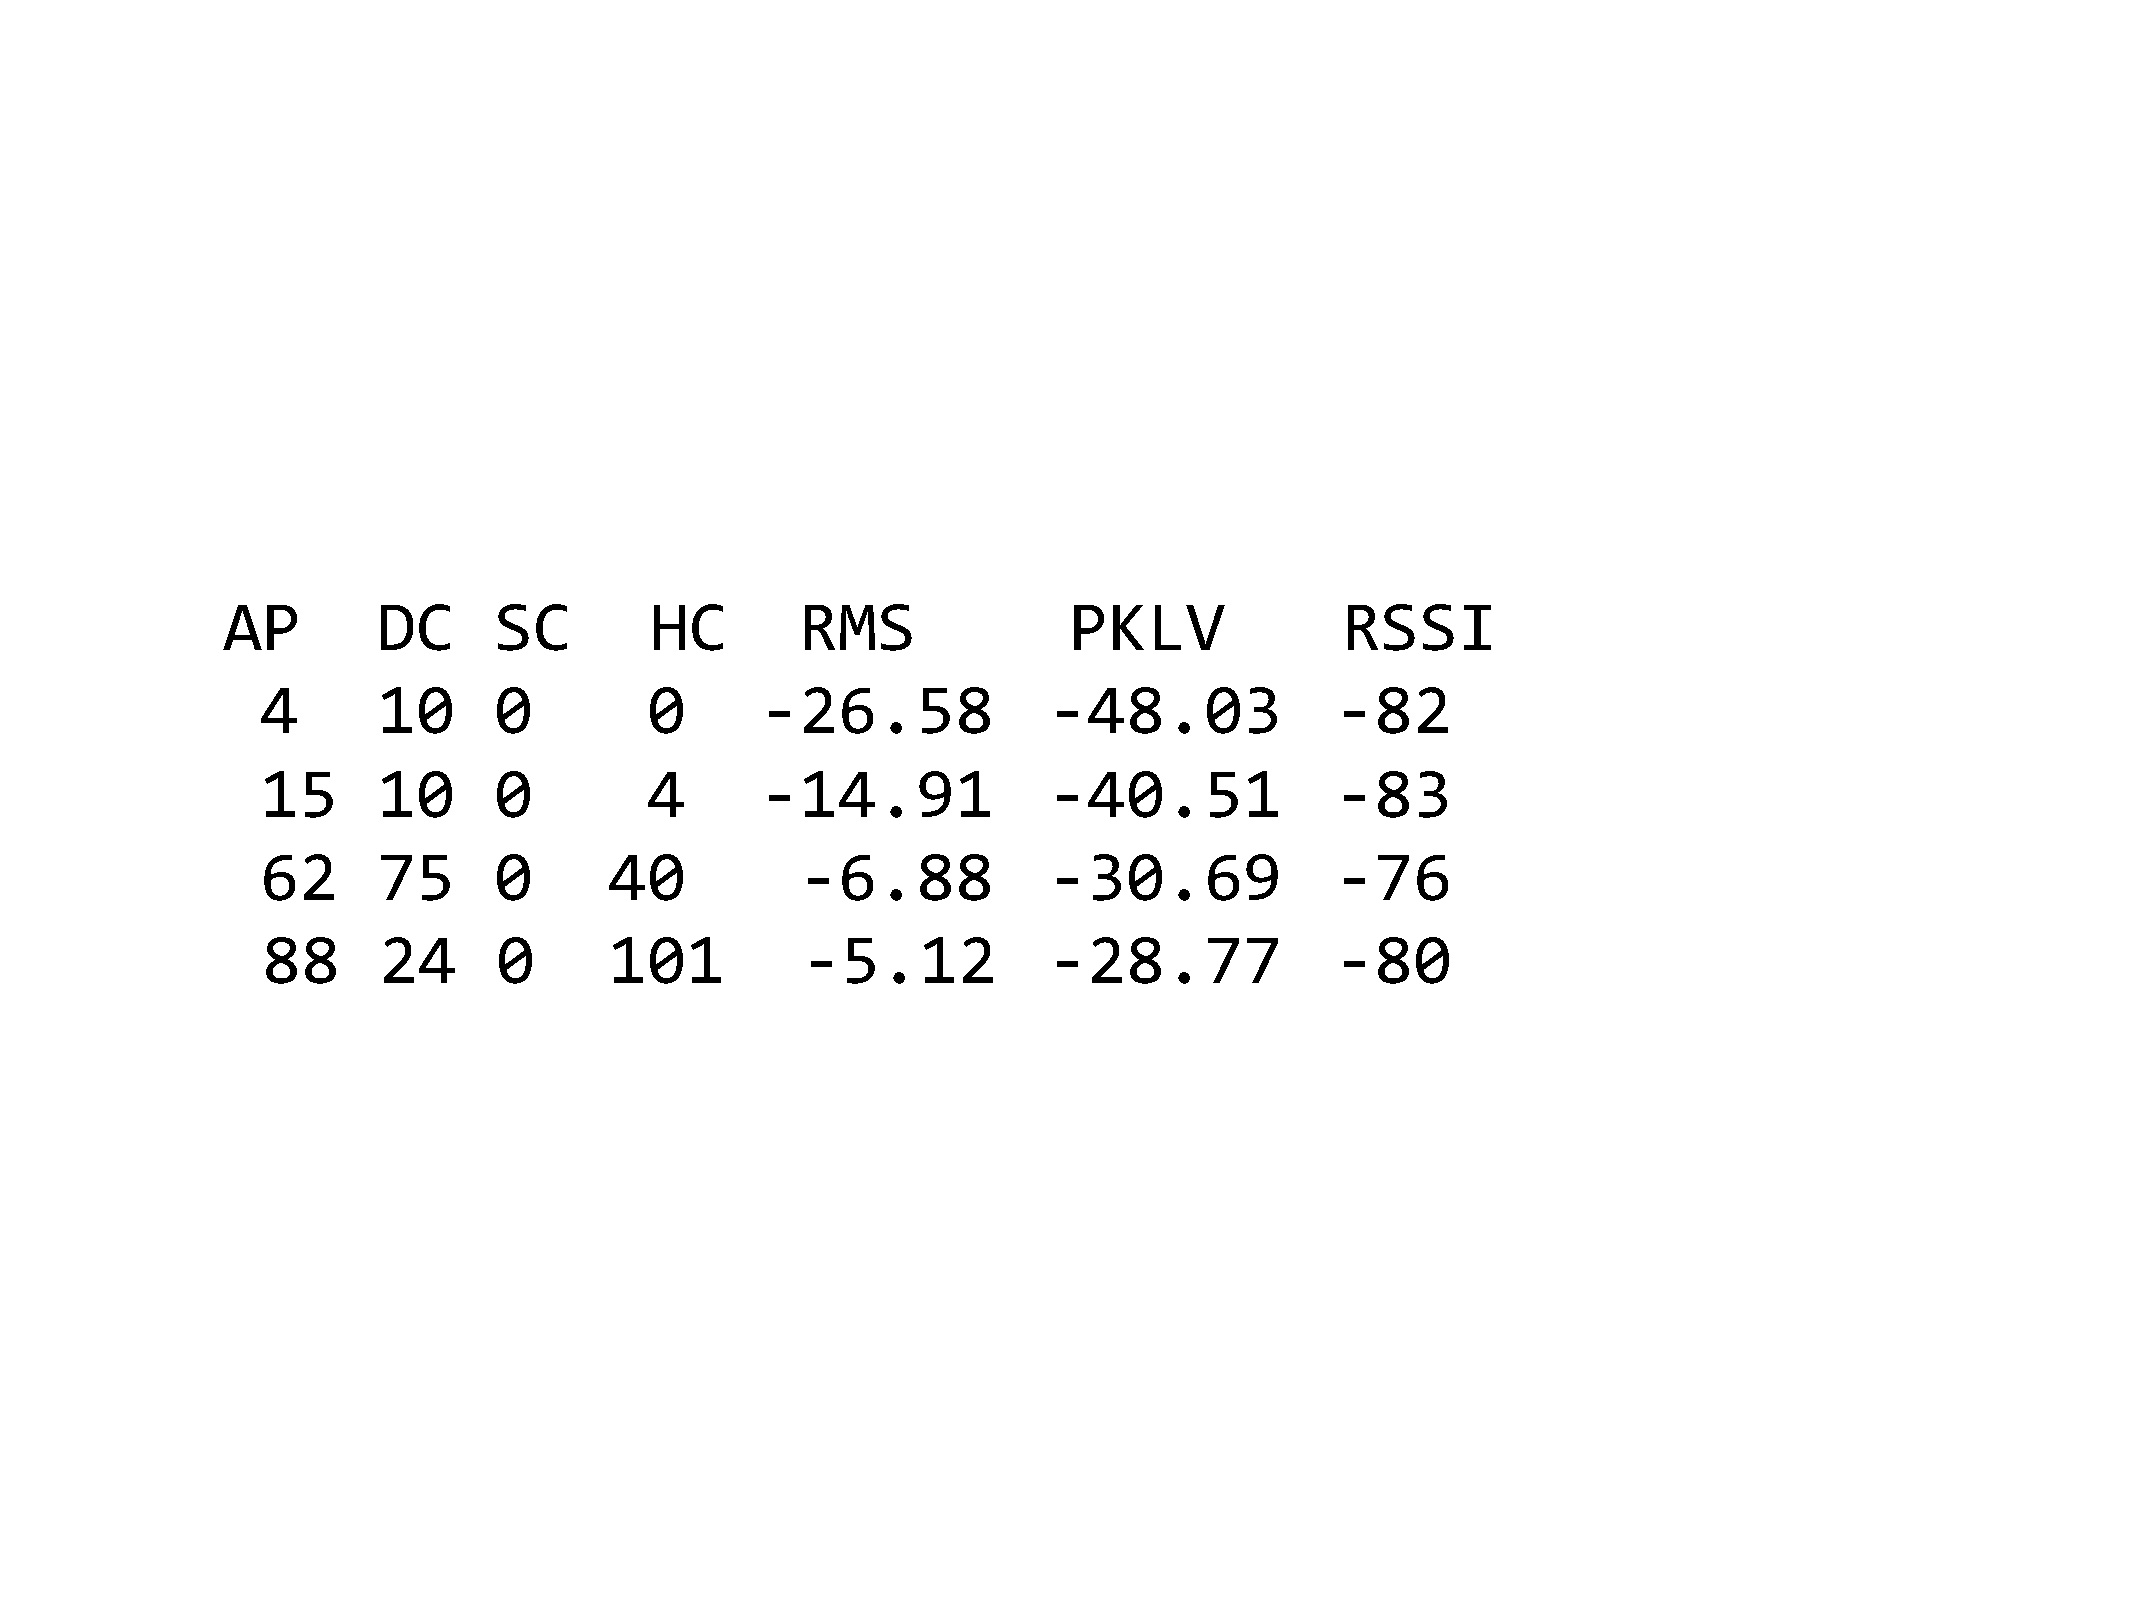
\includegraphics[width=0.7\textwidth]{./img/sensor-readings}
% 	\caption{Example of sensor readings.}
% 	\label{fig:scatterplot-matrix}
% \end{figure}

	\subsection{Linear Method for Regression} % (fold)
	\label{sub:linear_estimator}
	Linear regression is a method of modeling the relationship between a dependent variable and an explanatory (or predicting) variable by fitting a straight line across the data. A condition where there is only one explanatory variable is called simple linear regression, while multiple linear regression involves more than one explanatory variable. The result of linear regression is a linear function (or a model) with the explanatory variables as the parameters.

	To obtain a model with minimal error, we perform an exhaustive search for the best subsets of the predictors for predicting the dependent variable (head count or device count) in linear regression. We use \ac{RMSE} of 10-folds cross-validation to select the optimal model using the smallest value. \autoref{r-code-linear-regr}~displays the implementation of linear regression analysis. We implement linear regression using stepwise selection in R using \verb|caret|\footnote{\url{http://topepo.github.io/caret/index.html}} library.
	
	\begin{figure}[h]
		\begin{adjustwidth}{-1cm}{}
		\centering
		\subfloat[head count]{
			\label{fig:tuning-linear-headcount}{
				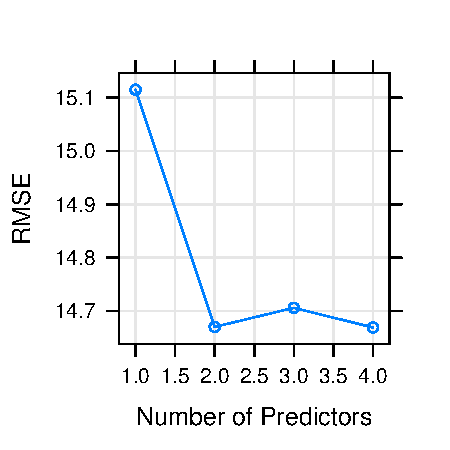
\includegraphics[width=0.65\textwidth]{./img/modeling/linear-regr-hc-small}
			}
		}
		\subfloat[device count]{
			\label{fig:tuning-linear-devicecount}{
				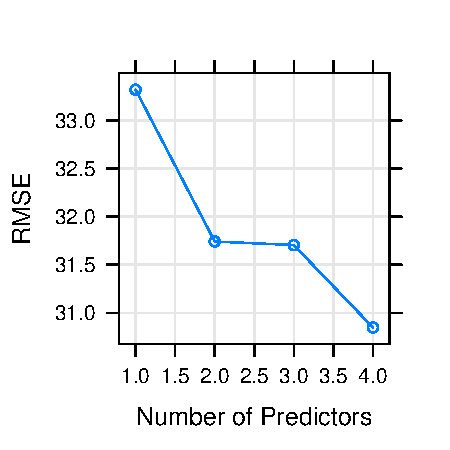
\includegraphics[width=0.65\textwidth]{./img/modeling/linear-regr-dc-small}
			}
		}
		\end{adjustwidth}
		\caption{Tuning linear regression using best subsets combination for head count (\ref{fig:tuning-linear-headcount}) and device count (\ref{fig:tuning-linear-devicecount}). The result indicates that using all predictors gives the best result, although in head count prediction using two predictors results in nearly the same error.}
		\label{fig:tuning-linear}
	\end{figure}

	\autoref{fig:tuning-linear}~presents the tuning result. For both head count and device count, using all four predictors results in optimal model. In head count prediction, using two predictors ($ap$ and $pklv$) yields in nearly identical \ac{RMSE} as using four predictors. Based on the tuning, we develop a linear model to predict the head count and device count. The linear model for head count prediction is 
	\begin{equation}
		hc=54.6750+0.6530ap-0.1091rms+0.7603pklv+0.3288rssi
	\end{equation}
	while the linear model for device count is 
	\begin{equation}
		dc=-367.901+2.021ap+1.138rms-1.880pklv-3.656rssi
	\end{equation}
	where $ap$, $rms$, $pklv$, and $rssi$ represent \ac{AP} count, \ac{RMS} and \ac{PKLV} of ambient noise recording, and \ac{RSSI} of scanned \ac{AP} respectively.
	% , using an efficient branch-and-bound algorithm. 

	% predictions and real result, show the graph as well, better using line graph
	% mention what is the training and what is the testing (better using 10 fold cross validation)
	

	% hc ==========================
	% Subset selection object
	% 4 Variables  (and intercept)
	%      Forced in Forced out
	% ap       FALSE      FALSE
	% rms      FALSE      FALSE
	% pklv     FALSE      FALSE
	% rssi     FALSE      FALSE
	% 1 subsets of each size up to 4
	% Selection Algorithm: forward
	%          ap  rms pklv rssi
	% 1  ( 1 ) "*" " " " "  " " 
	% 2  ( 1 ) "*" " " "*"  " " 
	% 3  ( 1 ) "*" " " "*"  "*" 
	% 4  ( 1 ) "*" "*" "*"  "*" 

	% Linear Regression with Stepwise Selection 

	% 459 samples
	%   4 predictor

	% No pre-processing
	% Resampling: Cross-Validated (10 fold, repeated 10 times) 
	% Summary of sample sizes: 414, 413, 412, 412, 412, 413, ... 
	% Resampling results across tuning parameters:

	%   nvmax  RMSE      Rsquared 
	%   1      15.11505  0.7320710
	%   2      14.67019  0.7467084
	%   3      14.70598  0.7455704
	%   4      14.66907  0.7467488

	% RMSE was used to select the optimal model using  the smallest value.
	% The final value used for the model was nvmax = 4. 

	% Call:
	% lm(formula = gt ~ ., data = phone_data_gt)

	% Coefficients:
	% (Intercept)           ap          rms         pklv         rssi  
	%     54.6750       0.6530      -0.1091       0.7603       0.3288 

	% \begin{figure}[h]
	% 	\centering
	% 	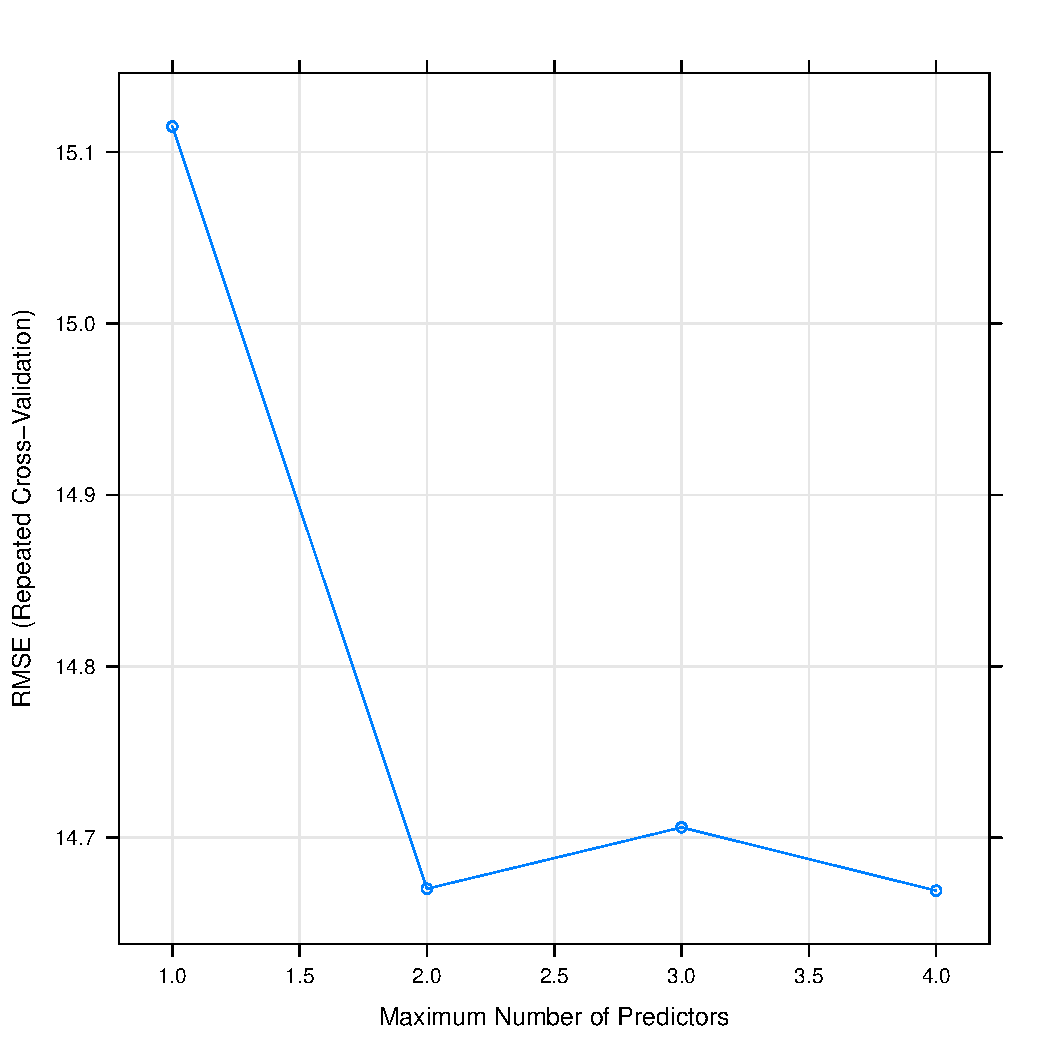
\includegraphics[width=0.9\textwidth]{./img/modeling/linear-regr-hc}
	% 	\caption{Tuning for linear regression.}
	% 	\label{fig:tuning-linear-hc}
	% \end{figure}

	% dc =========================
	% Subset selection object
	% 4 Variables  (and intercept)
	%      Forced in Forced out
	% ap       FALSE      FALSE
	% rms      FALSE      FALSE
	% pklv     FALSE      FALSE
	% rssi     FALSE      FALSE
	% 1 subsets of each size up to 4
	% Selection Algorithm: 'sequential replacement'
	%          ap  rms pklv rssi
	% 1  ( 1 ) "*" " " " "  " " 
	% 2  ( 1 ) "*" " " " "  "*" 
	% 3  ( 1 ) "*" " " "*"  "*" 
	% 4  ( 1 ) "*" "*" "*"  "*" 

	% Linear Regression with Stepwise Selection 

	% 459 samples
	%   4 predictor

	% No pre-processing
	% Resampling: Cross-Validated (10 fold, repeated 10 times) 
	% Summary of sample sizes: 414, 414, 413, 411, 414, 413, ... 
	% Resampling results across tuning parameters:

	%   nvmax  RMSE      Rsquared 
	%   1      33.32081  0.7752300
	%   2      31.74120  0.7979257
	%   3      31.70418  0.7990889
	%   4      30.84697  0.8103420

	% RMSE was used to select the optimal model using  the smallest value.
	% The final value used for the model was nvmax = 4.

	% Call:
	% lm(formula = pr ~ ., data = phone_data_pr)

	% Coefficients:
	% (Intercept)           ap          rms         pklv         rssi  
	%    -367.901        2.021        1.138       -1.880       -3.656 
	% \begin{figure}[h]
	% 	\centering
	% 	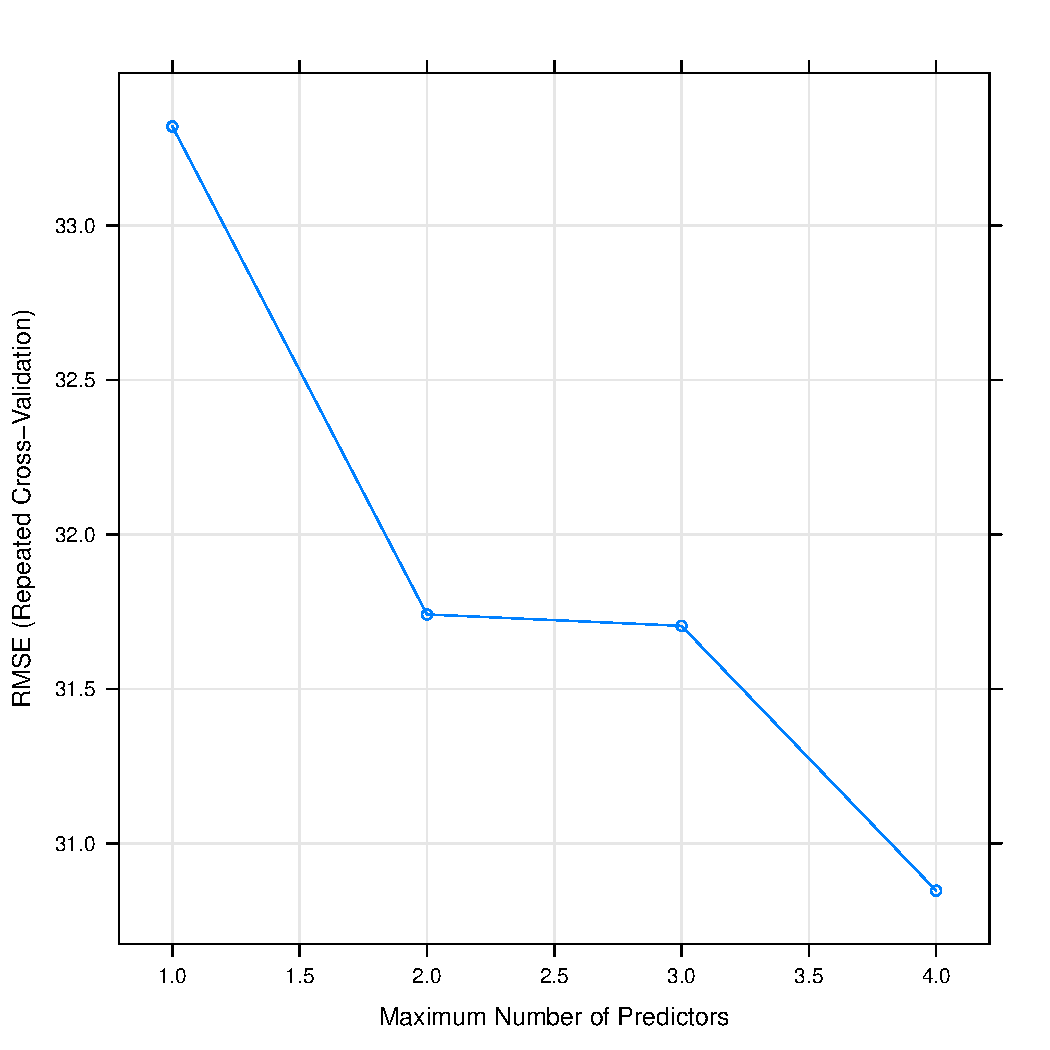
\includegraphics[width=0.9\textwidth]{./img/modeling/linear-regr-dc}
	% 	\caption{Tuning for linear regression.}
	% 	\label{fig:tuning-linear-dc}
	% \end{figure}

	\subsection{Non-Linear Method for Regression} % (fold)
	\label{sub:non_linear_estimator}
	We use \ac{k-NN} and \ac{SVM} as non-linear methods for regression. We tune the parameters of non-linear regression method to obtain the optimal model as well.

	% =====================knn===================================
	\ac{k-NN} is an algorithm that predicts numerical value based on similarity measure using distance function, e.g., euclidean, manhattan, or minkowski, of k-nearest neighbors of the predicted value. Generally, a large $k$ value is more accurate as it uses more neighbors to predict a new value. \ac{k-NN} is applicable for both classification and regression analysis.

	\begin{figure}[h]
		\begin{adjustwidth}{-1cm}{}
		\centering
		\subfloat[head count]{
			\label{fig:tuning-knn-hc}{
				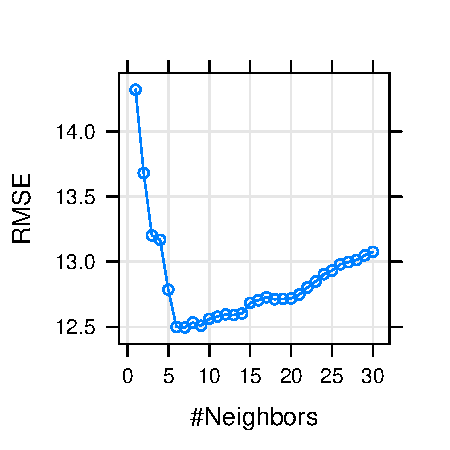
\includegraphics[width=0.65\textwidth]{./img/modeling/knn-hc-small}
			}
		}
		\subfloat[device count]{
			\label{fig:tuning-knn-dc}{
				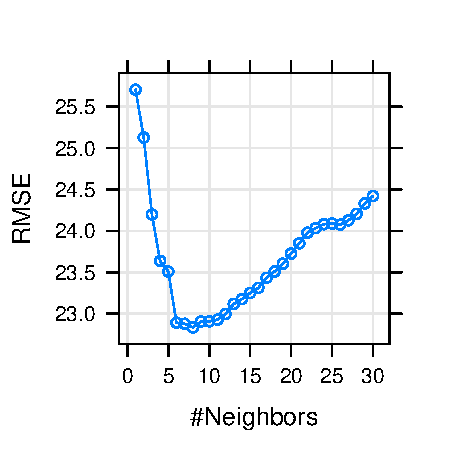
\includegraphics[width=0.65\textwidth]{./img/modeling/knn-dc-small}
			}
		}
		\end{adjustwidth}
		\caption{Tuning \ac{k-NN} using $1 \le k \le 30$ tuning parameter (\#Neighbors) for head count (\ref{fig:tuning-knn-hc}) and device count (\ref{fig:tuning-knn-dc}). For both estimation, optimal result is obtained when $5 \le k \le 10$. The optimal result is chosen at $k=7$ (head count) and $k=8$ (device count).}
		\label{fig:tuning-knn}
	\end{figure}

	We train and test \ac{k-NN} regression using $1 \le k \le 30$ as tuning parameter in R using \verb|caret|\footnote{\url{http://topepo.github.io/caret/index.html}} library. Like the linear regression analysis, we evaluate the model using 10-folds cross-validation and we use \ac{RMSE} to select the optimal model with lowest error. \autoref{r-code-knn}~displays the implementation of \ac{k-NN} regression.

	\autoref{fig:tuning-knn}~presents the tuning result. As we can see, the optimal models are obtained when $5 \le k \le 10$. According to~\autoref{fig:tuning-knn}, the highest error of both estimation is when $k=1$ and there is a increasing trend of error as $k$ goes up. We select the optimal model for head count and device count estimation when $k=7$ ($RMSE=12.49515$) and $k=8$ ($RMSE22.83321$), respectively.
	% hc ========================================================
	% k-Nearest Neighbors 

	% 459 samples
	%   4 predictor

	% No pre-processing
	% Resampling: Cross-Validated (10 fold, repeated 10 times) 
	% Summary of sample sizes: 414, 413, 412, 412, 412, 413, ... 
	% Resampling results across tuning parameters:

	%   k   RMSE      Rsquared 
	%    1  14.32195  0.7651252
	%    2  13.68100  0.7813994
	%    3  13.20218  0.7946098
	%    4  13.16852  0.7956532
	%    5  12.78561  0.8064473
	%    6  12.49908  0.8149187
	%    7  12.49515  0.8156143
	%    8  12.53433  0.8148571
	%    9  12.50869  0.8159582
	%    ...
	%   30  13.07611  0.7998607

	% RMSE was used to select the optimal model using  the smallest value.
	% The final value used for the model was k = 7. 

	%             Length Class      Mode     
	% learn       2      -none-     list     
	% k           1      -none-     numeric  
	% theDots     0      -none-     list     
	% xNames      4      -none-     character
	% problemType 1      -none-     character
	% tuneValue   1      data.frame list     
	% obsLevels   1      -none-     logical  

	% dc ========================================================
	% k-Nearest Neighbors 

	% 459 samples
	%   4 predictor

	% No pre-processing
	% Resampling: Cross-Validated (10 fold, repeated 10 times) 
	% Summary of sample sizes: 414, 414, 413, 411, 414, 413, ... 
	% Resampling results across tuning parameters:

	%   k   RMSE      Rsquared 
	%    1  25.70729  0.8686436
	%    2  25.12761  0.8746131
	%    3  24.19895  0.8823375
	%    4  23.63810  0.8880587
	%    5  23.50962  0.8894205
	%    6  22.89128  0.8950484
	%    7  22.87820  0.8953308
	%    8  22.83321  0.8958578
	%    9  22.90468  0.8955070
	%   10  22.90716  0.8953828
	%   ...
	%   30  24.42160  0.8851021

	% RMSE was used to select the optimal model using  the smallest value.
	% The final value used for the model was k = 8. 

	%             Length Class      Mode     
	% learn       2      -none-     list     
	% k           1      -none-     numeric  
	% theDots     0      -none-     list     
	% xNames      4      -none-     character
	% problemType 1      -none-     character
	% tuneValue   1      data.frame list     
	% obsLevels   1      -none-     logical 


	% =======================svm=============================================
	\ac{SVM} is an estimator that works by constructing support vectors (hyperplanes) that separate data according to a certain threshold. Most of the time, kernels, a set of mathematical functions, are used to remap the input data so that the data can be separated using a straight line instead of a complex curve. \ac{SVM} is also implementable for both classification and regression analysis.

	We implement \ac{SVM} regression using radial kernel along with $cost$ and $\epsilon$ as the tuning parameters. $cost$ and $\epsilon$ are used to apply a penalty to a prediction where the data are not correctly predicted. As used in \ac{k-NN}, we validate the model using 10-folds cross-validation. We use R with \verb|e1071| library\footnote{\url{https://cran.r-project.org/web/packages/e1071/index.html}}. \autoref{r-code-svm}~displays the implementation of \ac{SVM} regression.

	\begin{figure}[h]
		\begin{adjustwidth}{-1cm}{}
		\centering
		\subfloat[head count]{
			\label{fig:tuning-svm-hc}{
				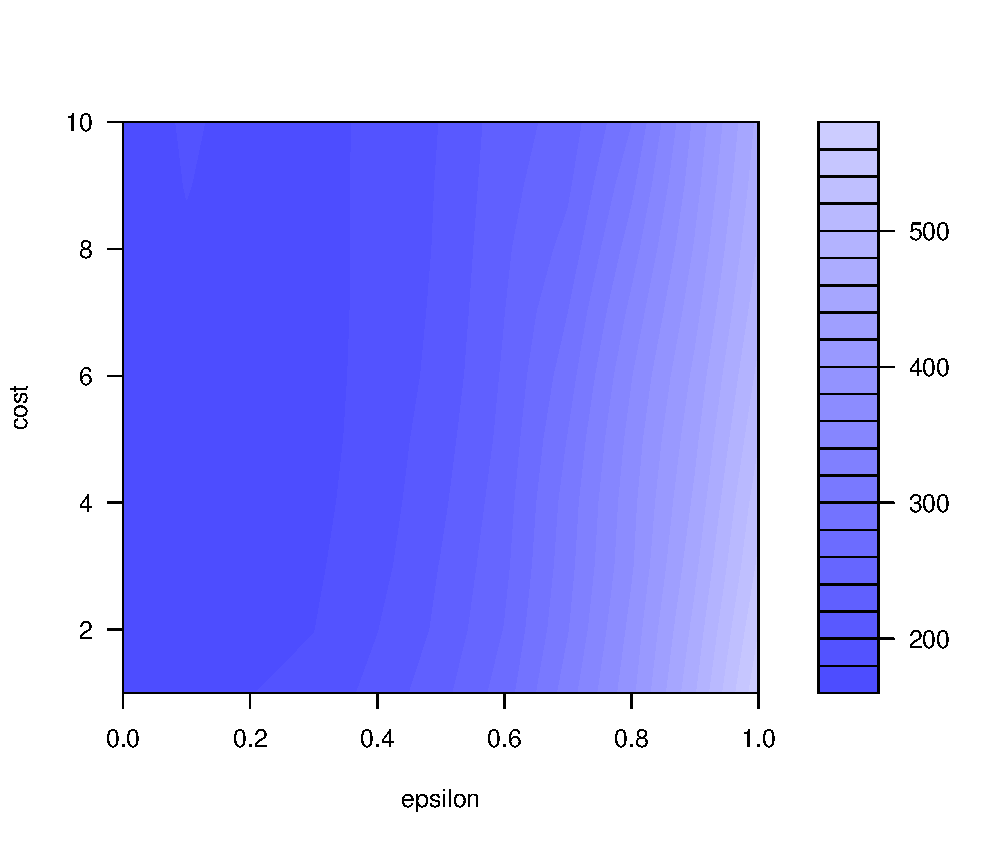
\includegraphics[width=0.65\textwidth]{./img/modeling/svm-hc}
			}
		}
		\subfloat[device count]{
			\label{fig:tuning-svm-dc}{
				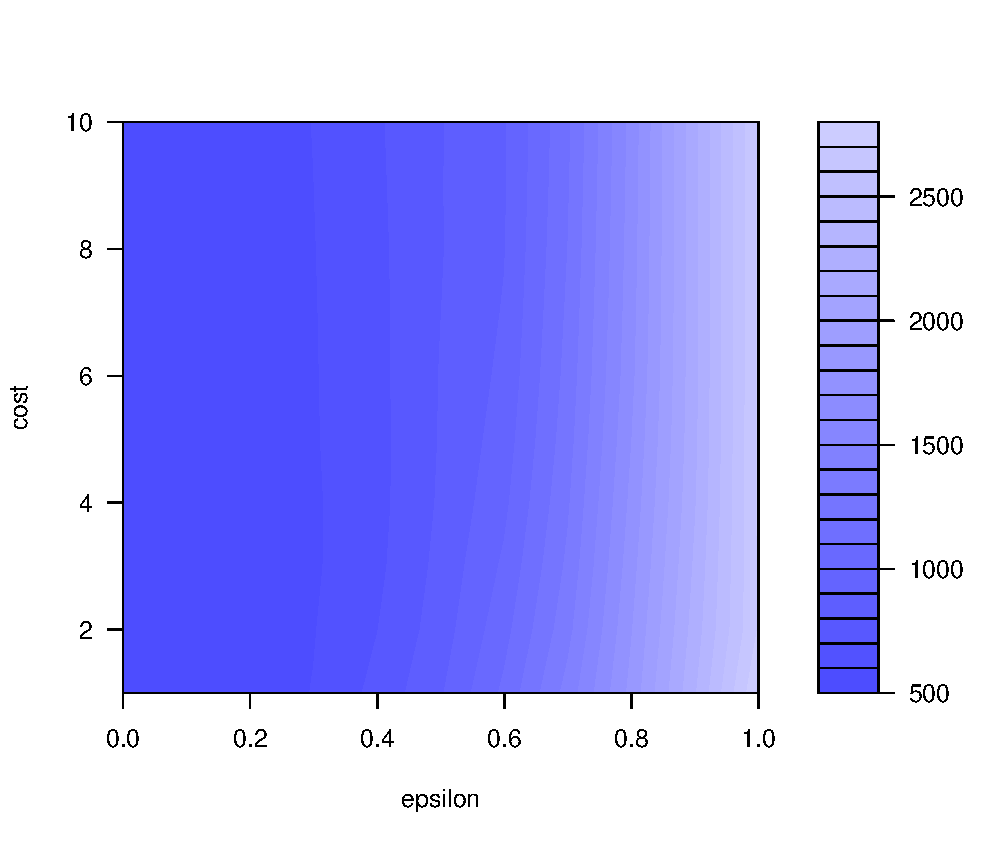
\includegraphics[width=0.65\textwidth]{./img/modeling/svm-dc}
			}
		}
		\end{adjustwidth}
		\caption{Tuning \ac{SVM} using $cost$ and $epsilon$ as the tuning parameters for head count (\ref{fig:tuning-svm-hc}) and device count (\ref{fig:tuning-svm-dc}) in R with \texttt{e1071} library. The performance is measured using \ac{MSE}. More optimal model is indicated by darker color, i.e., lower \ac{MSE}.}
		\label{fig:tuning-svm}
	\end{figure}

	We present the result of \ac{SVM} regression tuning in~\autoref{fig:tuning-svm}. The best performance for head count prediction is at 171.1065 with $\epsilon=0$ and $cost=3$, while for device count prediction is at 514.226 with $\epsilon=0$ and $cost=1$. We can also see a trend of increasing \ac{MSE} as the $epsilon$ increases.
	% hc============
	% Parameter tuning of 'svm':

	% - sampling method: 10-folds cross validation 

	% - best parameters:
	%  epsilon cost
	%        0    3

	% - best performance: 171.1065 


	% dc============
	% Parameter tuning of 'svm':

	% - sampling method: 10-folds cross validation 

	% - best parameters:
	%  epsilon cost
	%        0    1

	% - best performance: 514.226 

To summarize the regression analysis and to interpret the result, we use another approach to calculate the error, which has more intuitive interpretation. We use residual error, which can be formulated as
\begin{equation}\label{eq:residual-error}
	\bar { error } =\frac { 1 }{ n } \left( \sum _{ i=1 }^{ n }{ \left| { p }_{ i }-{ a }_{ i } \right|  }  \right) 
\end{equation}
where ${ p }_{ i }$ is the predicted value and ${ a }_{ i }$ is the actual value. As formulated in the equation, residual error shows mean of the difference between predicted and actual value. The optimal model has a residual error closer to zero.

\begin{table}[h]
\centering
\caption{Summary of regression analysis showing the range of the data and the residual error of each regression method.}
\label{tab:regression-summary}
\begin{tabular}{llllll}
\toprule
                   & \multicolumn{2}{c}{Value Range}                         & \multicolumn{3}{c}{Residual Error}                                                        \\
                   & \multicolumn{1}{c}{Min} & \multicolumn{1}{c}{Max} & \multicolumn{1}{c}{Linear} & \multicolumn{1}{c}{k-NN} & \multicolumn{1}{c}{SVM} \\ \midrule
Head count estimation   & 0                       & 115                     & 9.89                                  & 7.05                    & 7.06                    \\
Device count estimation & 0                       & 288                     & 23.81                                 & 13.14                   & 13.34                  \\ \bottomrule
\end{tabular}
\end{table}

\autoref{tab:regression-summary}~presents the summary of the regression analysis. Non-linear regression (\ac{k-NN} and \ac{SVM}) has better performance than the linear regression. \ac{k-NN} and \ac{SVM} do not have much difference of error for both head count and device count estimation. Device count estimation has wider value range and error compared to head count estimation.

% Plot the prediction graph in each cross validation round, then combined.
% Explain the result in percentage as well, instead of manual count. -> for the error in the modeling.
% plot the graph of head count (real vs predicted) vs parameters (ap count, or anything else)
% present the evaluation in people count and also percentage









\section{Discussion} % (fold)
\label{sec:discussion}
% In this chapter we look at to what extend these questions have been answered, what problems arose from answering them and what future directions this work can go in.

We discuss our findings in the present study in the following topics,


	% mac address randomization
	% mention about the randomization as well, that that might not a solution, mention the paper that comprehensively discuss about the randomization
	% explain that the IE (information elements on probe request) method is not really 100\% correct.
	% prove it by using LG nexus randomized and real probe request.
	% To avoid randomized mac, we use discretized monitoring, instead of doing it continuously for a long time, we did it in separate scanning interval.
	% Why dont you use 2 devices for separate purpose? one for probe request and one for access point.
	% When android is in energy saving mode, the OS prohibits any app for doing WiFi Scan or any other scan.
	% why the some SN disappear.

	% ambient noise
	We recorded ambient noise and extracted the peak-level (\ac{PKLV}) and root-mean-square(\ac{RMS}) of the recordings, which are highly correlated with $\rho=0.77$ (see~\autoref{fig:scatterplot-matrix}. Initially, we expect to see a strong correlation of ambient noise and the level of social density, i.e., the location which has high level of social density also has high value of ambient noise, but the result says otherwise. We can see in~\autoref{fig:scatterplot-matrix} that only the correlation of head count and peak level which is more than $0.5$ ($\rho=0.58$). The other correlations of social density level (head count or device count) and ambient noise (peak level or root-mean-square) are below $0.5$. In the scatter plot of~\autoref{fig:scatterplot-matrix}, we can also see that some of the low social density values (less than 20) have high ambient noise value as well (more than -20dB).

	However, we can also see in~\autoref{fig:scatterplot-matrix} that no high social density values (more than 50 for device count and 20 for head count) are below -30dB. We can conclude that high values of ambient noise mostly indicate a high level of social density. The line charts showing the peak level and root-mean-square of the ambient noise (\autoref{fig:audio-result-day1}, \autoref{fig:audio-result-day2}, \autoref{fig:audio-result-day3}, and \autoref{fig:audio-result-day4}) also support our conclusion. The graphs show that more crowded locations (Grote Markt and Paddepoel) have higher peak level or root-mean-square value than (Home and remote area) less crowded locations although some overlaps exist.

	Furthremore, microphone sensitivity also affects the result of ambient noise recording. We used laptop's built-in microphone to record the ambient noise. These microphones (and ones installed in smartphones) are attuned to a specific (and rather narrow) range of sound intensity.

	% https://support.biamp.com/General/Audio/Microphone_sensitivity
	% http://electronics.stackexchange.com/questions/59157/over-what-frequency-range-can-the-microphone-of-smartphone-receive-the-sound
	% http://www.makeuseof.com/tag/great-tips-recording-audio-smartphone-tablet/
	% http://www.scienceprog.com/long-range-directional-microphones-myth-and-reality/
	% http://www.epanorama.net/newepa/2014/09/08/sound-level-measuring-with-android-phone/
	% seems legit http://www.analog.com/library/analogdialogue/archives/46-05/understanding_microphone_sensitivity.html?doc=an-1328.pdf


	% social density estimation method
	We estimate the crowd count as a first approximation of the ground truth because it is known that getting the ground truth of crowd density in public spaces is difficult~\cite{thesis041}. We used time-lapse image based, works by manually counting heads in the images, and WiFi's probe request based technique, works by counting unique \ac{MAC} addresses. Both methods rely on predefined assumptions.

	Although probe request based estimation is promising, some drawbacks are also present. In this method, we are not able to distinguish the type of devices, i.e., whether it is a smartphone, tablets, or computers. Although one mostly brings a smartphone~\cite{thesis047}, which means we can deduce that a smartphone means a person present, there is also a possibility that one brings more devices or no devices at all.

	Furthermore, WiFi based technique is able to detect object through walls, which could be good or bad depending on the perspective. In indoor social density estimation, this is a bad approximation because WiFi might detect some people but in fact there are no people at all within a room as they are located in another room nearby. This is a potential threat, for instance if  our method detects some people but actually no one is present in the room. However, in outdoor social density estimation, WiFi based technique performs better than image based technique, as WiFi can see people through an obstacle, while image-based cannot. To sum up, we have to be more careful in doing indoor monitoring. We can also combine with ambient recording to see whether there is a noise inside a room, as empty room is mostly quite. 
	
	Compared to the probe request based estimation, time-lapse image based technique cannot detect people through walls or buildings. This may be the reason why the image based technique detects less people than the WiFi based technique (see~\autoref{fig:total-population}). Furthermore, image based technique relies heavily on assumptions, especially when vehicles, e.g., buses or cars, are captured in the image, as vehicles have very limited visual appearance of the people inside. We assume that there are a person in a car and five people in a bus. This assumptions may slightly bias the result.

	% scanning timing
	We tested the effect on scanning time to investigate whether scanning time can potentially affect the outcomes. An interesting findings about the scanning time are shown in~\autoref{fig:time-effect}. We can see that the device count in each scanning time has different outcome, while the \ac{AP} count remains stable around 100 no matter when the scanning was performed. When we scanned the surroundings in the morning (09:00h), the device count is less than the \ac{AP} count, as there were not so many people present. However, the trend changed when we performed the scanning at 12:00h. The device count surpasses the \ac{AP} count. We can also see an increasing trend at scanning time performed at 15:00h and decreasing trend at 18:00h.
	According to the trends, there might be lower device count than \ac{AP} count at night.

	The findings presented in~\autoref{fig:time-effect} indicates that we also have to note the scanning time of the surroundings when the present study is implemented because different scanning time might have a very different outcome.



	% mention about the correlation, talk about why why why and explain subjectively
	The parameter which has a strong correlation with head count or device count (the proxy of social density) is the \ac{AP} count, as shown in the top right of~\autoref{fig:scatterplot-matrix}. The correlation coefficients of \ac{AP} count vs device count, \ac{AP} count vs head count, and device count vs head count are 0.87, 0.85, and 0.86, respectively. We present in detail the correlation of head count, device count, and \ac{AP} count in~\autoref{sub:ap_and_social_density_correlation}.

	As we can see in~\autoref{fig:ap-dc-scatterplot}, \autoref{fig:ap-hc-scatterplot}, and \autoref{fig:hc-dc-scatterplot}, the lower social density data, as at home or remote area, seems to be more concentrated than higher social density data, as at Paddepoel or Grote Markt, and the higher social density data is widely spread. However, this does not mean that frequency of high social density value is bigger than the low social density value. In fact, we have more data for lower social density than higher social density, as shown in the histograms of \ac{AP}, \ac{DC}, and \ac{HC} in~\autoref{fig:scatterplot-matrix}.

	If we look at~\autoref{fig:ap-dc-scatterplot}, \autoref{fig:ap-hc-scatterplot}, and \autoref{fig:hc-dc-scatterplot}, the data may be also use to perform a sort of localization, as each location show different pattern. We could possibly infer where the location is using features of the data, although further study is required to support this opinion.

	% present the result of each location. and compare within days.
	
	Furthermore, we expect at the beginning that the number of \ac{AP} follows the fluctuation of the number of people in a certain location, as people might bring their own portable WiFi transmitter to assemble an ad-hoc \ac{AP}, which will add up the number of \ac{AP} available in the location. However, this turned out to be a rare situation, as we do not see any trend between number of people and \ac{AP} count, as shown in time based experiment~\autoref{fig:time-effect}.

	Moreover, if we see at the line chart, there is a fluctuation of \ac{AP} count, although actually it should be the same or stable across the time. This fluctuation might be caused by the instability of radio transmission that may affect the signal strength of the WiFi \ac{AP} and thus making some \ac{AP}s some not detected.
	
	Another interesting finding is that, it turned out that several \ac{AP}s are using the same \ac{SSID}, e.g., eduroam. This makes user see only one \ac{AP} available, in fact, those \ac{AP} are using different \ac{MAC} address.
	

	







	\subsection{Limitation of the Proposed Method} % (fold)
	\label{sub:limitation_of_the_present_study}
	The proposed method has some limitations that limit the implementation of this social density estimation.
	% #1: location: range, indoor outdoor
	The first limitation is the location. The proposed work only works on places where WiFi \ac{AP} use is not restricted, i.e., people are free to set up their own WiFi AP. Some locations where the use of WiFi is restricted exist, for instance, University of Groningen complex, where eduroam is the only the available AP and the occupants are discouraged to install their own AP. If we collect data from this location, we will possibly get very static value of \ac{AP} count.

	Furthermore, our dataset consists of data collected from four different location. This dataset represents the situation of selected locations but possibly not for other locations, as other locations may have different characteristics. For instance, in developing countries or other locations where the use of WiFi are not common, the number of \ac{AP} in a public area may be much lower than what the data explains.

	As we mainly work with WiFi, the range of the proposed social density follows the maximum WiFi coverage of the smartphone, which extends roughly from 20 to 50 meters. This range may be good or bad depending on the context. For outdoor situation, this range gives a good approximation as it is considerably broad enough to count social density. However, this range may be too broad for indoor implementation. For instance, we may get a result that says there are 20 people in total, but in fact there is only five or even less people in the room. This is because WiFi also detects people outside the room. However, we can also combine the result with ambient noise recording, as empty room are usually more quite.

	% Use wigle to explain that this could not be generalized. Mention comparison of one place and another place. in other cities or contries.

	% #2: time
	The other limitation is the time. Our dataset consists of data collected in daytime, ranging from 08:15h to 14:45h. Using this dataset, we are only able to approximate the level of social density if the new data is captured during the same time frame. If the new data is taken outside the time frame, our dataset is not capable to tell the level of social density. This fact is based on the time of scanning investigation described in~\autoref{ssub:effect_of_scanning_time} and \autoref{sub:effect_of_scanning_time}.
	

	

	

	


	



% conclusion
As a conclusion, 
- be aware about generalization of this method
Explain that using classification might give better accuracy that regression.
also use % https://wigle.net/ database of public WiFi
Explain by conclusion, not using whole data
effect of day
effect of location
effect of scanning time
put it in a whole picture
signal strength: WiFi and probe request
Combine with GPS location if there is no sound detected.
the setting may vary in cities or even countries.
- other free interpretation about the data.
becarefull when we are doing indoor monitoring.
we have to look back to the data to inspect what happened.
conclude from all other paragraphs (part of the discussion)

We also select daytime as the preferred scanning time because that is the time when most crowd are observable. This implies that our collected data resemble only daytime duration, meaning that conclusion might only be able to deduct for daytime.

generalization of this method requires further investigation in more locations, hence more data.

% Question: Does weather affect WiFi performance?

%*****************************************
%*****************************************
%*****************************************
%*****************************************
%*****************************************
